\documentclass[12pt, a4paper]{article}

% Acentuação
\usepackage[utf8]{inputenc}
\usepackage[portuguese]{babel}
\usepackage[T1]{fontenc}

% Configurando as margens
\usepackage[top = 3cm, bottom = 2cm, left = 3cm, right = 2cm, includefoot]{geometry}
% Indentação do parágrafo
\setlength{\parindent}{2cm}
% Espaçamento entre parágrafo e texto
\setlength{\parskip}{1em}
% Espaçamento entre linhas
\renewcommand{\baselinestretch}{1.5}
% Identar o primeiro parágrafo das seções
\usepackage{indentfirst}
% Para colocar texto entre $$ com \text{oi}
\usepackage{amsmath}
% Para usar listas com estilos específicos
\usepackage{enumerate}
% Para utilizar imagens
\usepackage{graphicx}
% Posicionamento de imagem
\usepackage{float}
% Para símbolo de permilagem com \textperthousand em modo texto
\usepackage{textcomp}
% Notação de conjuntos: $\mathbb{N, Z, Q, R, C}$ e para usar símbolos como >=
\usepackage{amssymb}

% Header e footer
\usepackage{fancyhdr}
\pagestyle{fancy}
\fancyhead{}
\fancyfoot{}
\fancyhead[R]{\thepage}
\renewcommand{\headrulewidth}{0pt}

% \uptau
\usepackage{upgreek}

\begin{document}

	\input{Título.tex}
	
	\section{Álgebra linear}
		\subsection{Autovalores e autovetores}
		Seja $A=(a_{ij})\in\mathbb{M}_n(\mathbb{R})$. Dizemos que um valor $\lambda\in\mathbb{R}$ é um autovalor de $A$ se o sistema
\begin{equation} \label{eq:auto1}
\begin{pmatrix}a_{11} & \dots & a_{1n}\\ \vdots & \vdots & \vdots\\ a_{n1} & \dots & a_{nn}\\ \end{pmatrix}\cdot\begin{bmatrix}x_1\\ \vdots\\ x_n\\ \end{bmatrix}=\lambda\cdot\begin{bmatrix}x_1\\ \vdots\\ x_n\\ \end{bmatrix}
\end{equation}

tiver uma solução não nula. Para um tal autovalor $\lambda$, cada solução de \eqref{eq:auto1} será chamada de autovetor de $A$ associado a $\lambda$ (ou simplesmente, um autovetor de $A$).

\textbf{Notação}: Se $\lambda$ for um autovalor de uma matriz $A$, indicamos por $V(\lambda)$ ao conjunto de todos os autovetores de $A$ associados a $\lambda$ (isto é, o conjunto solução do sistema \eqref{eq:auto1}).

\textbf{Exemplo}: Considere uma matriz $A=\begin{pmatrix}-1 & 2\\ 2 & -4\\ \end{pmatrix}$

Queremos encontrar um valor $\lambda\in\mathbb{R}$ (se isso for possível) tal que o sistema
\begin{equation} \label{eq:autoex1}
\begin{pmatrix}-1 & 2\\ 2 & -4\\ \end{pmatrix}\cdot\begin{bmatrix}x_1\\x_2\\ \end{bmatrix}=\lambda\cdot\begin{bmatrix}x_1\\x_2\\ \end{bmatrix}
\end{equation}

tenha soluções não nulas. Observe que podemos escrever
$$\begin{bmatrix}x_1\\x_2\\ \end{bmatrix}=\begin{pmatrix}1 & 0\\0 & 1\\ \end{pmatrix}\cdot\begin{bmatrix}x_1\\x_2\\ \end{bmatrix}$$

Daí, a relação \eqref{eq:autoex1} pode ser escrita como
$$\begin{pmatrix}-1 & 2\\2 & -4\\ \end{pmatrix}\cdot\begin{bmatrix}x_1\\x_2\\ \end{bmatrix}=\lambda\cdot\begin{pmatrix}1 & 0\\0 & 1\\ \end{pmatrix}\cdot\begin{bmatrix}x_1\\x_2\\ \end{bmatrix}=\begin{pmatrix}\lambda & 0\\0 & \lambda\\ \end{pmatrix}\cdot\begin{bmatrix}x_1\\x_2\\ \end{bmatrix}$$

Com isso,
$$\begin{pmatrix}\lambda & 0\\0 & \lambda\\ \end{pmatrix}\cdot\begin{bmatrix}x_1\\x_2\\ \end{bmatrix}-\begin{pmatrix}-1 & 2\\2 & -4\\ \end{pmatrix}\cdot\begin{bmatrix}x_1\\x_2\\ \end{bmatrix}=\begin{bmatrix}0\\0\\ \end{bmatrix}$$
$$\left[\begin{pmatrix}\lambda & 0\\0 & \lambda\\ \end{pmatrix}-\begin{pmatrix}-1 & 2\\2 & -4\\ \end{pmatrix}\right]\cdot\begin{bmatrix}x_1\\x_2\\ \end{bmatrix}=\begin{bmatrix}0\\0\\ \end{bmatrix}$$
\begin{equation} \label{eq:autoex1a}
\begin{pmatrix}
\lambda+1 & -2\\-2 & \lambda+4\\ \end{pmatrix}\cdot\begin{bmatrix}x_1\\x_2\\ \end{bmatrix}=\begin{bmatrix}0\\0\\ \end{bmatrix}
\end{equation}

Nosso problema se reduz a encontrar um valor $\lambda\in\mathbb{R}$ tal que o sistema \eqref{eq:autoex1a} tenha uma solução não nula. Existe um teorema que diz que um tal sistema homogêneo tem solução não nula se e somente se o determinante de sua matriz de coeficientes for zero. Com isto, existirá um $\lambda$ como queremos se e somente se
$$0=\det\begin{pmatrix}\lambda+1 & -2\\-2 & \lambda+4\\ \end{pmatrix}=(\lambda+1)\cdot(\lambda+4)-2\cdot2=\lambda(\lambda+5)$$

isto é, quando $\lambda=0$ ou $\lambda=-5$. Esses valores serão os autovalores de $A$. Para cada autovalor deve-se achar os autovetores correspondentes. Substitui-se o respectivo valor de $\lambda$ encontrado em \eqref{eq:autoex1a} e resolve-se os sistemas correspondentes.

Para $\lambda=0$, o sistema \eqref{eq:autoex1a} será:
$$\begin{pmatrix}1 & -2\\-2 & 4\\ \end{pmatrix}\cdot\begin{bmatrix}x_1\\x_2\\ \end{bmatrix}=\begin{bmatrix}0\\0\\ \end{bmatrix}$$

ou
$$\begin{cases}x_1-2x_2=0\\-2x_1+4x_2=0\\ \end{cases}$$

Como a 2ª equação é a 1ª multiplicada por -2, a solução do sistema é a resolução da 1ª equação. Não é difícil ver que o conjunto solução desse sistema é $\{(2a,\;a):a\in\mathbb{R}\}$.

Para $\lambda=-5$, o sistema \eqref{eq:autoex1a} será:
$$\begin{pmatrix}-4 & -2\\-2 & -1\\ \end{pmatrix}\cdot\begin{bmatrix}x_1\\x_2\\ \end{bmatrix}=\begin{bmatrix}0\\0\\ \end{bmatrix}$$

ou
$$\begin{cases}-4x_1-2x_2=0\\-2x_1-x_2=0\\ \end{cases}$$

que tem conjunto solução igual a $\{(a,\;-2a):a\in\mathbb{R}\}$.
		
		\subsection{Polinômio característico}
		Um autovalor real de uma matriz $A=(a_{ij})\in\mathbb{M}_n(\mathbb{R})$, $n\geqslant1$, é um valor $\lambda\in\mathbb{R}$ tal que o sistema
\begin{equation} \label{eq:polcar1}
\begin{pmatrix}a_{11} & \dots & a_{1n}\\ \vdots & \vdots & \vdots\\a_{n1} & \dots & a_{nn}\\ \end{pmatrix}\cdot\begin{bmatrix}x_1\\ \vdots \\ x_n\\ \end{bmatrix}=\lambda\cdot\begin{bmatrix}x_1\\ \vdots \\ x_n\\ \end{bmatrix}
\end{equation}

tenha uma solução não nula. Inicialmente, observe que
$$\lambda\cdot\begin{bmatrix}x_1\\x_2\\ \vdots\\x_n\\ \end{bmatrix}=\lambda\cdot\begin{pmatrix}1 & 0 & \dots & 0\\0 & 1 & \dots & 0\\ \vdots & \vdots & & \vdots\\0 & 0 & \dots & 1\\ \end{pmatrix}\cdot\begin{bmatrix}x_1\\x_2\\ \vdots\\x_n\\ \end{bmatrix}=\begin{pmatrix}\lambda & 0 & \dots & 0\\0 & \lambda & \dots & 0\\ \vdots & \vdots & & \vdots\\0 & 0 & \dots & \lambda \end{pmatrix}\cdot\begin{bmatrix}x_1\\x_2\\ \vdots\\x_n\\ \end{bmatrix}$$

Com isso, tem-se que \eqref{eq:polcar1} é equivalente a
$$
\begin{pmatrix}\lambda & 0 & \dots & 0\\0 & \lambda & \dots & 0\\ \vdots & \vdots & & \vdots\\0 & 0 & \dots & \lambda \end{pmatrix}\cdot\begin{bmatrix}x_1\\x_2\\ \vdots\\x_n\\ \end{bmatrix}-\begin{pmatrix}a_{11} & a_{12} & \dots & a_{1n}\\a_{21} & a_{22} & \dots & a_{2n}\\ \vdots & \vdots & & \vdots\\a_{n1} & a_{n2} & \dots & a_{nn}\\ \end{pmatrix}\cdot\begin{bmatrix}x_1\\x_2\\ \vdots\\x_n\\ \end{bmatrix}=\begin{bmatrix}0\\0\\ \vdots\\0\\ \end{bmatrix}$$

ou
\begin{equation} \label{eq:polcar2}
\begin{pmatrix}\lambda-a_{11} & -a_{12} & \dots & -a_{1n}\\-a_{21} & \lambda-a_{22} & \dots & -a_{2n}\\ \vdots & \vdots & & \vdots\\-a_{n1} & -a_{n2} & \dots & \lambda-a_{nn}\\ \end{pmatrix}\cdot\begin{bmatrix}x_1\\x_2\\ \vdots\\x_n\\ \end{bmatrix}=\begin{bmatrix}0\\0\\ \vdots\\0\\ \end{bmatrix}
\end{equation}

A matriz de coeficientes do sistema \eqref{eq:polcar2} pode então ser escrita como $(\lambda\cdot I-A)$ que obviamente pertence a $\mathbb{M}_n(\mathbb{R})$. O sistema \eqref{eq:polcar2} terá uma solução não nula se e somente se $\det(\lambda\cdot I-A)=0$.

O polinômio característico de uma matriz $A\in\mathbb{M}_n(\mathbb{R})$ é o polinômio $p_a(t)=\det(t\cdot I-A)$.

O problema de encontrar os autovalores de uma matriz $A$ transforma-se em achar as possíveis raízes do polinômio $p_a(t)$. Como sabe-se que um polinômio de grau $n$ possui no máximo $n$ raízes distintas, conclui-se que uma matriz $A\in\mathbb{M}_n(\mathbb{R})$ possui no máximo $n$ autovalores distintos. Uma vez encontradas as raízes de $p_a(t)$, o cálculo dos autovetores associados a elas se reduz à solução de sistemas lineares.

\textbf{Exemplo:} Calcule os autovalores e os autovetores da matriz:
$$A=\begin{pmatrix}-1 & 3 & 0\\-3 & 5 & 0\\1 & 1 & 2\\ \end{pmatrix}$$

Primeiramente, seu polinômio característico:
$$p_a(t)=\det\begin{pmatrix}t+1 & -3 & 0\\3 & t-5 & 0\\-1 & -1 & t-2\\ \end{pmatrix}=(t+1)\cdot(t-5)\cdot(t-2)-[-9\cdot(t-2)]=$$
$$=(t-2)\cdot[(t+1)\cdot(t-5)+9]=(t-2)\cdot(t^2-5t+t-5+9)=$$
$$(t-2)\cdot(t^2-4t+4)=(t-2)\cdot{(t-2)}^2={(t-2)}^3$$

Logo, o único autovalor da matriz $A$ é 2 (pois 2 é a raíz tripla de $p_a(t)$). Agora, calcula-se os autovetores associados a 2, isto é, a solução do sistema:
$$\begin{pmatrix}3 & -3 & 0\\3 & -3 & 0\\-1 & -1 & 0\\ \end{pmatrix}\cdot\begin{bmatrix}x\\y\\z\\ \end{bmatrix}=\begin{bmatrix}0\\0\\0\\ \end{bmatrix}$$

ou
$$\begin{cases}3x-3y=0\\3x-3y=0\\-x-y=0\\ \end{cases}$$

Escalonando o sistema, tem-se:
$$\begin{cases}3x-3y=0\\-6y=0\\ \end{cases}$$

O que implica em $x=y=0$.

Observa-se que qualquer valor de $z\in\mathbb{R}$ induz uma solução do sistema do tipo $(0,\;0,\;z)=z(0,\;0,\;1)$. Logo, os autovetores associados a 2 são os múltiplos de $(0,\;0,\;1)$.

\textbf{Exemplo:} Considere uma matriz quase idêntica à do exemplo anterior (a diferença está no valor $a_{31}$).
$$A=\begin{pmatrix}-1 & 3 & 0\\-3 & 5 & 0\\-1 & 1 & 2\\ \end{pmatrix}$$

Seu polinômio característico é (também) $p_a(t)={(t-2)}^3$. Já que na multiplicação nas diagonais onde está o $a_{31}$ existe o número zero. Logo, 2 é o único autovalor de $A$. Para o cálculo dos autovetores, tem-se:
$$\begin{pmatrix}3 & -3 & 0\\3 & -3 & 0\\1 & -1 & 0\\ \end{pmatrix}\cdot\begin{bmatrix}x\\y\\z\\ \end{bmatrix}=\begin{bmatrix}0\\0\\0\\ \end{bmatrix}$$

ou
$$\begin{cases}3x-3y=0\\3x-3y=0\\x-y=0\\ \end{cases}$$

É fácil ver que o conjunto solução do sistema será o conjunto solução da equação $x-y=0$, o que implica que $x=y$. De novo, o valor de $z$ pode ser qualquer e portanto, tem-se que os autovetores de $A$ são vetores do tipo $(x,\;x,\;z)=x(1,\;1,\;0)+z(0,\;0,\;1)$, com $x, z\in\mathbb{R}$.
	
	\section{Cálculo diferencial e integral}
		\subsection{Teorema do Valor Médio}
		\input{Calculo-diferencial-e-integral/Teorema-do-valor-médio.tex}	
	
		\subsection{Regra de l'Hôspital}
		\input{Calculo-diferencial-e-integral/Regra-de-l'Hôspital.tex}

		\subsection{Produtos indeterminados}
		Quando $f(x) \rightarrow 0$ e $g(x) \rightarrow \infty$ (ou $-\infty$) quando $x \rightarrow a$, o limite do produto $f \cdot g$ é considerado indeterminado do tipo $0 \cdot \infty$.
	
Há uma disputa entre as funções e precisamos saber quem ganhará. Se $f$ ganhar, o limite é $0$, se $g$ ganhar, o limite é $\infty$ (ou $-\infty$). Podendo ainda haver um equilíbrio e o limite tender a um número específico.

Podemos resolver reescrevendo $$\lim_{x \to a} f \cdot g$$ como $$\lim_{x \to a} \frac{f}{1/g} \text{ ou } \lim_{x \to a} \frac{g}{1/f}$$

Isso converte o produto indeterminado em outro do tipo $0/0$ ou $\infty/\infty$, fazendo com que seja possível aplicar a Regra de l'Hôspital.
		
		\subsection{Diferenças indeterminadas}
		\input{Calculo-diferencial-e-integral/Diferenças-indeterminadas.tex}
	
		\subsection{Potências indeterminadas}
		\input{Calculo-diferencial-e-integral/Potências-indeterminadas.tex}
		\input{Calculo-diferencial-e-integral/Potências-indeterminadas-Exemplo.tex}
	
		\subsection{Esboço de curvas}
		\input{Calculo-diferencial-e-integral/Esboço-de-curvas.tex}
		
		\subsection{Derivação implícita}
		Consiste na derivação de ambos os lados da equação em relação a $x$ e, então, na resolução da equação isolando $y'$ ou $\displaystyle\frac{dy}{dx}$.
		\begin{enumerate}
	\item Calcular $\displaystyle\frac{dy}{dx}$ para $x^2+y^2=25$
		$$\frac{d}{dx}(x^2+y^2)=\frac{d}{dx}25$$
		$$2x+2y\frac{dy}{dx}=0$$
		$$\frac{dy}{dx}=-\frac{x}{y}$$
	\item Encontre uma equação da tangente ao círculo $x^2+y^2=25$ no ponto (3, 4)
		
		No ponto (3, 4), tem-se $x=3$ e $y=4$:
		$$\frac{dy}{dx}=-\frac{3}{4}$$
		$$y-y_0=m(x-x_0)$$
		$$y-4=-\frac{3}{4}(x-3)$$
		Ou $$3x+4y=25$$
	\item Calcular $y'$ para $x^3+y^3=6xy$ (Fólio de Descartes)
		$$x^3+y^3=6xy$$
		$$3x^2+3y^2y'=6(xy'+y\cdot1)$$
		$$x^2+y^2y'=2xy'+2y$$
		$$y^2y'-2xy'=2y-x^2$$
		$$y'(y^2-2x)=2y-x^2$$
		$$y'=\frac{2y-x^2}{y^2-2x}$$
	\item Calcular $y'$ para $\sin(y+x)=y^2\cos x$
		$$\sin(y+x)=y^2\cos x$$
		$$\cos(y+x)(y'+1)=y^2(-\sin x)+\cos x\cdot2yy'$$
		Agrupando termos semelhantes
		$$\cos(y+x)+y^2\sin x=\cos x\cdot(2yy')-\cos(y+x)y'$$
		$$\cos(y+x)+y^2\sin x=y'(\cos x\cdot2y-\cos(y+x))$$
		$$y'=\frac{\cos(y+x)+y^2\sin x}{\cos x\cdot2y-\cos(y+x)}$$
	\item Calcular $y''$ para $x^4+y^4=16$
		$$x^4+y^4=16$$
		$$4x^3+4y^3y'=0$$
		$$y'=-\frac{4x^3}{4y^3}=-\frac{x^3}{y^3}$$
		Derivando $y'$ pela Regra do Quociente:
		$$y''=\frac{d}{dx}\left(-\frac{x^3}{y^3}\right)=-\left(\frac{y^3\cdot3x^2-x^3\cdot3y^2y'}{(y^3)^2}\right)$$
		Substituindo $y'$ na equação acima:
		$$-\left(\frac{y^3\cdot3x^2-x^3\cdot3y^2\left[-\displaystyle\frac{x^3}{y^3}\right]}{y^6}\right)$$
		$$-\frac{3(x^2y^4+x^6)}{y^7}=-\frac{3x^2(y^4+x^4)}{y^7}$$
		
		Podendo ainda ser simplificada, pois $x^4+y^4=16$
		$$-\frac{3x^2(16)}{y^7}=-\frac{48x^2}{y^7}$$
\end{enumerate}
		
	\section{Resistência dos materiais}
		\subsection{Tensão e deformação - carregamento axial}
		Considerando uma barra de comprimento $L$ e seção transversal uniforme, e chamando-se de $\delta$ sua deformação sob uma carga axial $P$:

// Inserir imagem

Define-se a \textit{deformação específica normal} $\varepsilon$ da barra como sendo a \textit{deformação por unidade de comprimento}:
\begin{equation}\label{eq:def-espec}
	\varepsilon=\frac{\delta}{L}
\end{equation}

Em barra de seção transversal variável, a deformação específica normal é definida:
\begin{equation}
	\varepsilon=\lim_{\Delta x\rightarrow0}\frac{\Delta\delta}{\Delta x}=\frac{d\delta}{dx}
\end{equation}

// Inserir imagem

A porção inicial do diagrama tensão-deformação é uma linha reta. Isto significa que para pequenas deformações a tensão é diretamente proporcional à deformação:
\begin{equation}\label{eq:leidehooke}
	\sigma=E\varepsilon
\end{equation}

Esta relação é conhecida como Lei de Hooke e o coeficiente $E$ como \textit{módulo de elasticidade longitudinal} do material. A maior tensão para a qual a Equação~\eqref{eq:leidehooke} se aplica é a \textit{tensão de proporcionalidade} do material.
		
		\subsection{Deformações de barras sujeitas a cargas axiais}		
		Tratando-se de deformação elástica, se uma barra de comprimento $L$ e seção transversal uniforme de área $A$ é submetida a uma carga $P$, axial e centrada em sua extremidade, a correnpondente deformação é, a partir da junção de que $\sigma=F/A$ e das Equações~\eqref{eq:def-espec} e~\eqref{eq:leidehooke}:
$$\varepsilon=\frac{\delta}{L}$$
$$\sigma=E\varepsilon$$

Sua união,
$$\varepsilon=\frac{\sigma}{E}=\frac{P}{AE}$$

Portanto,
\begin{equation}\label{eq:def-elastica}
	\delta=\frac{PL}{AE}
\end{equation}

Se a barra for carregada em vários pontos ou consiste em várias partes com seções transversais diferentes, e ainda, possivelmente, de diferentes materiais, a deformação $\delta$ da barra deve ser expressa como o somatório das deformações nas várias partes:
\begin{equation}
	\delta=\sum_i\frac{P_iL_i}{A_iE_i}
\end{equation}
		
		\subsection{Problemas envolvendo variação de temperatura}
		Tomando uma barra $AB$, homogênea e de seção transversal uniforme, apoiada em uma superfície lisa horizontal. Se for aumentada a temperatura da barra em um valor $\Delta T$, nota-se que ela se alonga de um valor $\delta_T$ que é proporcional tanto à variação de temperatura quanto ao comprimento da barra $L$. Tem-se, então:
\begin{equation}\label{eq:def-total}
	\delta_T=\alpha(\Delta T)L
\end{equation}

Onde $\alpha$ é a constante característica do material, chamada de \textit{coeficiente de dilatação térmica}. Como $L$ e $\delta_T$ são expressos em unidades de comprimento, $\alpha$ representa uma quantidade \textit{por grau C} ou \textit{por grau F}, dependendo de como a temperatura é expressada.

À deformação total $\delta_T$ está relacionada uma deformação específica $\varepsilon_T=\delta_T/L$. Reescrevendo a Equação~\eqref{eq:def-total}:
\begin{equation}
	\varepsilon_T=\alpha(\Delta T)
\end{equation}

Onde $\varepsilon_T$ é chamada de \textit{deformação térmica específica}, uma vez que é causada por variação de temperatura na barra. No caso considerado não há tensões relacionadas com a deformação $\varepsilon_T$.

\begin{figure}[H]
	\begin{center}
	\caption{Aumento de comprimento devido o acréscimo de temperatura.}
    	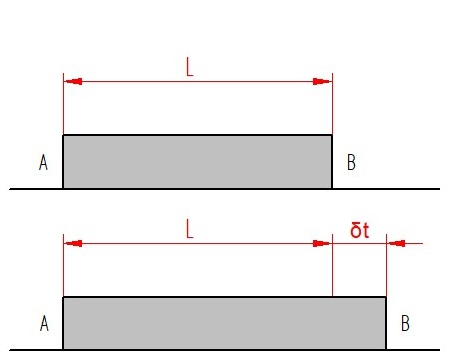
\includegraphics[width=0.5\textwidth]{Resistencia-dos-materiais/Imagens/Variacao-de-temperatura.jpg}
	\end{center}
\end{figure}

Agora, um caso específico. Considerando uma barra $AB$ de comprimento $L$, colocada entre dois anteparos fixos, separados por uma distância $L$. Elevando-se $\Delta T$, o alongamento da barra é nulo, pois os anteparos impedem qualquer deformação. Sendo a barra homogênea e de seção uniforme, a deformação específica em qualquer ponto é $\varepsilon=\delta_t/L$, também nula. Entretanto, para evitar o alongamento da barra, os anteparos vão aplicar sobre ela as forças $P$ e $P'$ após a elevação da temperatura. É criado um estado de tensão na barra (sem que ocorram deformações específicas).

\begin{figure}[H]
	\begin{center}
	\caption{Aumento de temperatura sem deformação.}
    	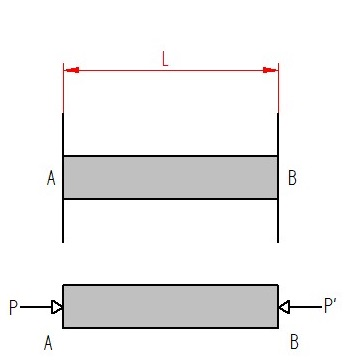
\includegraphics[width=0.5\textwidth]{Resistencia-dos-materiais/Imagens/Variacao-de-temperatura-sem-deformacao.jpg}
	\end{center}
\end{figure}

Na tentativa de se calcular a tensão $\sigma$ criada pela variação de temperatura, verifica-se que o problema é estaticamente indeterminado. É necessário calcular a força $P$, levando em conta as condições de alongamento nulo da barra. Utilizando o método da superposição, retira-se o anteparo $B$ que restringe a deformação da barra. Ela então se alonga livremente com variação de temperatura $\Delta T$. Sabe-se que pela Equação~\eqref{eq:def-total}, o alongamento correspondente é:
$$\delta_T=\alpha(\Delta T)L$$

Aplicando-se na extremidade $B$ da barra a força $P$ que representa a reação superabundante e, utilizando a Equação~\eqref{eq:def-elastica}:
$$\delta_P=\frac{PL}{AE}$$

Como a deformação total deve ser nula, tem-se:
$$\delta=\delta_T+\delta_P=\alpha(\Delta T)L+\frac{PL}{AE}=0$$
$$\alpha(\Delta T)+\frac{P}{AE}=0$$
$$\frac{AE\alpha(\Delta T)+P}{AE}=0$$
$$P=-AE\alpha(\Delta T)$$

Portanto, a tensão atuante na barra devido à variação de temperatura $\Delta T$ é:
$$\sigma=\frac{P}{A}=-E\alpha(\Delta T)$$

Esse caso e a observação anterior sobre ausência de deformações específicas \textit{se aplicam no caso de barra se seção transversal uniforme e material homogêneo}. Qualquer outro problema envolvendo variações de temperatura em estruturas impedidas de se deformarem deve ser analisado dentro de suas características. De qualquer modo, pode-se smepre considerar separadamente as deformações provocadas pela variação de temperatura e pelas reações superabundantes e superpor os resultados.	
		
		\subsection{Estado plano de tensão}
		\input{Resistencia-dos-materiais/Estado-plano-de-tensão.tex}
		
\end{document}